\subsection{Flip Flops tipo D}
Un flip-flop puede mantener un estado binario indefinidamente (en tanto se alimente al circuito), hasta que una señal de entrada le indique que debe cambiar de estado.
El flip-flop D es un dispositivo secuencial que se utiliza para almacenar un bit de información. El flip-flop D se puede construir a partir de un flip-flop tipo JK, conectando las entradas J y K a un nivel lógico alto. La tabla de verdad de un flip-flop D es la siguiente:

\begin{table}[h]
    \centering
    \begin{tabular}{|c|c|c|}
        \hline
        \textbf{D} & \textbf{CLK} & \textbf{Q} \\ \hline
        0         & 0           & 0         \\ \hline
        0         & 1           & 0         \\ \hline
        1         & 0           & 1         \\ \hline
        1         & 1           & 1         \\ \hline
    \end{tabular}
\end{table}

Esto quiere decir que si la entrada D es 0, la salida Q no cambia, sin importar el valor de CLK. Si la entrada D es 1, la salida Q toma el valor de D en el flanco de subida de CLK.    

\subsubsection{Registros}
Un registro consiste en un grupo de flip-flops. Estos pueden contener, además, compuertas lógicas. Las compuertas lógicas se utilizan para efectuar la transición de información entre los flip-flops.

Cada flip-flop puede almacenar un bit de información. Un registro de n bits consiste en un grupo de n flip-flops capaces de almacenar n bits de información binaria.

\begin{enumerate}
    \item Si el problema a resolver depende de alguna entrada externa que diferencie entre diferentes funcionamientos, generalmente se utilizan multiplexores para seleccionar la entrada adecuada.
    \item Si se habla de un registro de desplazamiento, se puede utilizar un multiplexor para seleccionar la entrada adecuada.
    \item Cuando se habla de paridad se debe tener en cuenta que el bit de paridad se suelen colocar compuertas XOR en la entrada de datos.
\end{enumerate}

\subsubsection{Contadores}
Un contador es un circuito secuencial que genera una secuencia de números binarios. Los contadores se pueden clasificar en dos tipos: contador síncrono y contador asíncrono.

\begin{enumerate}
    \item \textbf{Contador asíncrono:} En un contador asíncrono, la entrada de reloj de cada flip-flop es la salida del flip-flop anterior. La entrada de reloj del primer flip-flop es la señal de reloj del sistema. La salida de un contador asíncrono es la salida de los flip-flops.
    \item \textbf{Contador síncrono:} En un contador síncrono, la entrada de reloj de todos los flip-flops es la misma señal de reloj del sistema. La entrada de reloj de todos los flip-flops es la misma señal de reloj del sistema. La salida de un contador síncrono es la salida de los flip-flops.
\end{enumerate}

\subsubsection{Circuitos secuenciales}
Un circuito secuencial es un circuito que contiene elementos de almacenamiento, como flip-flops, y compuertas lógicas. Un circuito secuencial es de la forma:

\begin{figure}[h]
    \centering
    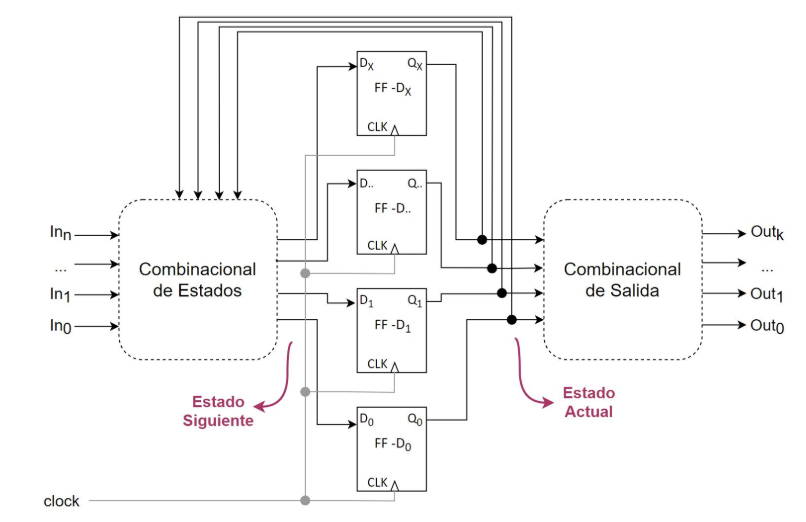
\includegraphics[scale=0.8]{img/sec.png}
    \caption{Diagrama de un circuito de memoria}
\end{figure}
\begin{itemize}
    \item \textbf{Combinacional de estados:} Se basa en un circuito combinacional, ya sea mediante el uso de decodificadores, multiplexores, etc. Son encargados de generar las señales de estados que se van a almacenar en los flip-flops. \textbf{Toman como entrada los estados actuales y las entradas del sistema.}
    \item \textbf{Memoria de estados:} Se basa en un conjunto de flip-flops que almacenan los estados del sistema. \textbf{Se encargan de almacenar los estados generados por el circuito combinacional.}
    \item \textbf{Combinacional de salidas:} Se basa en un circuito combinacional que genera las salidas del sistema. \textbf{Toman como entrada los estados almacenados en la memoria de estados y generan las salidas del sistema.}
\end{itemize}

Las salidas de los flip-flops se conectan a las entradas de los flip-flops, de esta manera se logra que el circuito se comporte de manera secuencial.